\subsection{Absorption Wavelength Prediction Across Data Regimes}
% ------------------------------------------------------------------
% Absorption: multi-panel comparison across datasets
% ------------------------------------------------------------------
\begin{figure*}[t]
  \centering
  \includegraphics[width=0.8\linewidth]{figures/abs_multipanel_bootstrap_ci.png}
  \caption{\textbf{Peak absorption wavelength ($\lambda_{\max}$) prediction across Deep4Chem, ChemFluor, and DSSCDB.} Test RMSE versus training set size $N$ for random (top row) and Bemis--Murcko scaffold (bottom row) splits. Each column corresponds to a dataset and uses dataset-specific $N$ values. Error bars indicate 95\% percentile bootstrap confidence intervals for the test RMSE, computed by resampling test molecules with replacement (2000 replicates). Models marked with an asterisk incorporate TD-DFT–derived HOMO--LUMO gap information.}
  \label{fig:multipanel-n-vs-rmse}
\end{figure*}

\paragraph{Consistent hybrid advantage in low-to-mid data regimes.}
Figure~\ref{fig:multipanel-n-vs-rmse} reports test RMSE as a function of training set size $N$ for peak absorption wavelength ($\lambda_{\max}$) prediction. Across datasets and split types, the hybrid D-MPNN$\rightarrow$XGBoost model generally outperforms the end-to-end D-MPNN in low-to-mid data regimes ($N \leq 1000$), with the strongest gains appearing under scaffold splits and in the smaller training-size settings. The magnitude of this effect is summarized in Table~\ref{tab:hybrid_pct_improvement}; for Deep4Chem, we observe an average RMSE reduction of \textbf{6.5\% for random splits} and \textbf{9.2\% for scaffold splits} within the $50 \leq N \leq 1000$ range.

We attribute this overall advantage to the structural regularization of gradient-boosted trees. In data-limited regimes, high-dimensional FFN heads are prone to high-variance estimation and overfitting. In contrast, the tree-based structure of XGBoost enforces simpler decision boundaries within the learned embedding space, acting as a robust regularization prior. This effect is most pronounced under scaffold splits (Deep4Chem), where the distribution shift is largest (see Figure~\ref{fig:split-validation}). As data availability increases ($N > 1000$) or distribution shift decreases (DSSCDB), the end-to-end model receives sufficient signal to stabilize the head, and the performance gap closes.


\begin{table}[h]
\centering
\caption{Percentage RMSE improvement of the Hybrid model (frozen D-MPNN embeddings $\rightarrow$ XGBoost) relative to the end-to-end D-MPNN. Positive values indicate lower RMSE for the Hybrid model.}
\label{tab:hybrid_pct_improvement}
\begin{tabular}{lcccccc}
\toprule
 & \multicolumn{2}{c}{\textbf{DEEP4CHEM}} & \multicolumn{2}{c}{\textbf{CHEMFLUOR}} & \multicolumn{2}{c}{\textbf{DSSCDB}} \\
\cmidrule(lr){2-3} \cmidrule(lr){4-5} \cmidrule(lr){6-7}
$N$ 
& Rand (\%) & Scaf (\%) 
& Rand (\%) & Scaf (\%) 
& Rand (\%) & Scaf (\%) \\
\midrule
50   & \textbf{+5.7} & \textbf{+7.7} & \textbf{+10.8} & \textbf{+9.8}  & \textcolor{gray}{-1.6} & \textbf{+5.4} \\
100  & \textbf{+8.8} & \textbf{+10.6}& \textbf{+9.8}  & \textbf{+15.6} & \textbf{+2.8} & \textbf{+3.5} \\
250  & \textbf{+7.5} & \textbf{+7.6} & \textbf{+8.0}  & \textbf{+6.0}  & \textbf{+2.7} & \textbf{+3.5} \\
1000 & \textbf{+4.1} & \textbf{+11.0}& +1.2           & \textbf{+5.4}  & \textbf{+5.4} & +0.4 \\
Max $N^{\dagger}$ 
     & \textbf{+8.0} & +1.3           & +0.8           & \textcolor{gray}{-28.8} & \textbf{+9.3} & \textbf{+7.0} \\
\bottomrule
\multicolumn{7}{l}{\footnotesize $^\dagger$ Max $N$: DEEP4CHEM (11,816), CHEMFLUOR (3,072), DSSCDB (1,376).}
\end{tabular}
\end{table}

\paragraph{Benchmarking against physical and classical baselines.}
Fingerprint-based baselines exhibit the expected hierarchy: augmenting Morgan fingerprints with physicochemical descriptors improves performance, but both graph-based models (End-to-End and Hybrid) generally outperform these fixed-feature approaches once $N \geq 250$.

In the ultra-low data regime ($N \leq 100$), physics-informed baselines utilizing TD-DFT--derived HOMO--LUMO gaps (dashed lines) remain the most robust, particularly under scaffold splits. This highlights the necessity of strong physical inductive biases when experimental supervision is scarce. However, as $N$ increases, the D-MPNN-based models rapidly overtake the DFT-augmented baselines. This crossover indicates that the learned graph representations eventually capture higher-order structural information that exceeds the predictive content of a single vacuum-phase orbital gap. The graph models achieve this accuracy without the computational overhead of calculating DFT descriptors at inference time.

\paragraph{Comparison to Multi-Fidelity Frameworks.}
We benchmark our approach against the multi-fidelity D-MPNN ensemble of Greenman \textit{et al.}~\cite{greenman2022multi}. Using identical preprocessing and scaffold splits on Deep4Chem, our Hybrid model achieves a test RMSE (27.5~nm) comparable to their reported ChempropMultiFidelity result (27.47~nm).

The Greenman framework relies on auxiliary pretraining with TD-DFT excitation energies. Generating this auxiliary data for the $\sim$5,800 molecules in Deep4Chem requires an estimated $10^5$ core-hours of quantum-chemical calculations (RDKit $\rightarrow$ xTB $\rightarrow$ DFT $\rightarrow$ TD-DFT) (K. Greenman, personal communication, Feb 11, 2026). Our results demonstrate that such expensive pretraining may not be necessary for comparable performance on this benchmark. By using a hybrid architecture with implicit regularization, we achieve comparable accuracy using purely experimental supervision, without the need for a quantum-chemical pipeline.

\paragraph{Summary: Regime-dependent tradeoffs and practical workflows.}
These results reveal a clear regime-dependent tradeoff. In the data-scarce limits ($N \lesssim 1000$) typical of experimental screening, the hybrid architecture offers meaningful accuracy gains; as dataset size increases, this advantage diminishes and fully joint optimization becomes competitive.
The computational cost of fitting an XGBoost head on fixed embeddings is negligible compared to the cost of training the D-MPNN encoder itself. Consequently, given a trained D-MPNN, practitioners can extract the learned embeddings and fit a lightweight XGBoost head with virtually no overhead. This ensures optimal performance in the low-data limit without sacrificing the scalability of the end-to-end model as data grows.
We note that this hybrid advantage is most pronounced for absorption; as detailed in the Supporting Information, results for emission prediction were less systematic, consistent with the greater physical complexity of excited-state relaxation and solvent reorganization effects, which are harder to capture in a static representation.

\subsection{Variance Decomposition}

Figure~\ref{fig:multipanel-n-vs-rmse} shows that model hybridization is most beneficial in low-$N$ regimes; we next ask which sources of stochasticity drive this behaviour. We use the variance decomposition framework introduced in Methods to identify which sources of stochasticity dominate predictive performance across data regimes, and to explain the observed convergence of hybrid and end-to-end models at scale.

\paragraph{Head sensitivity and selection.}
To isolate variability attributable solely to the regression head, we evaluated three models (MLP, RF, and XGBoost) on a fixed, pretrained D-MPNN encoder. As shown in the Supporting Information (Figure~\ref{fig:fixed-model}), XGBoost typically provided the strongest mean performance with minimal variance, motivating its adoption as the standard head for the hybrid architecture used throughout this work.

\paragraph{Regime-dependent variance decomposition.}
Figure~\ref{fig:var-decomp} presents the variance decomposition on Deep4Chem as a function of training set size. In small-data regimes ($N \leq 250$), a substantial proportion of predictive variability ($\sim$20--30\%) is attributable to the downstream head. This implies that under limited supervision, the mapping from molecular representation to property is underdetermined; the choice of regression model and its optimization significantly impacts generalization.

\begin{figure}[ht]
  \centering
  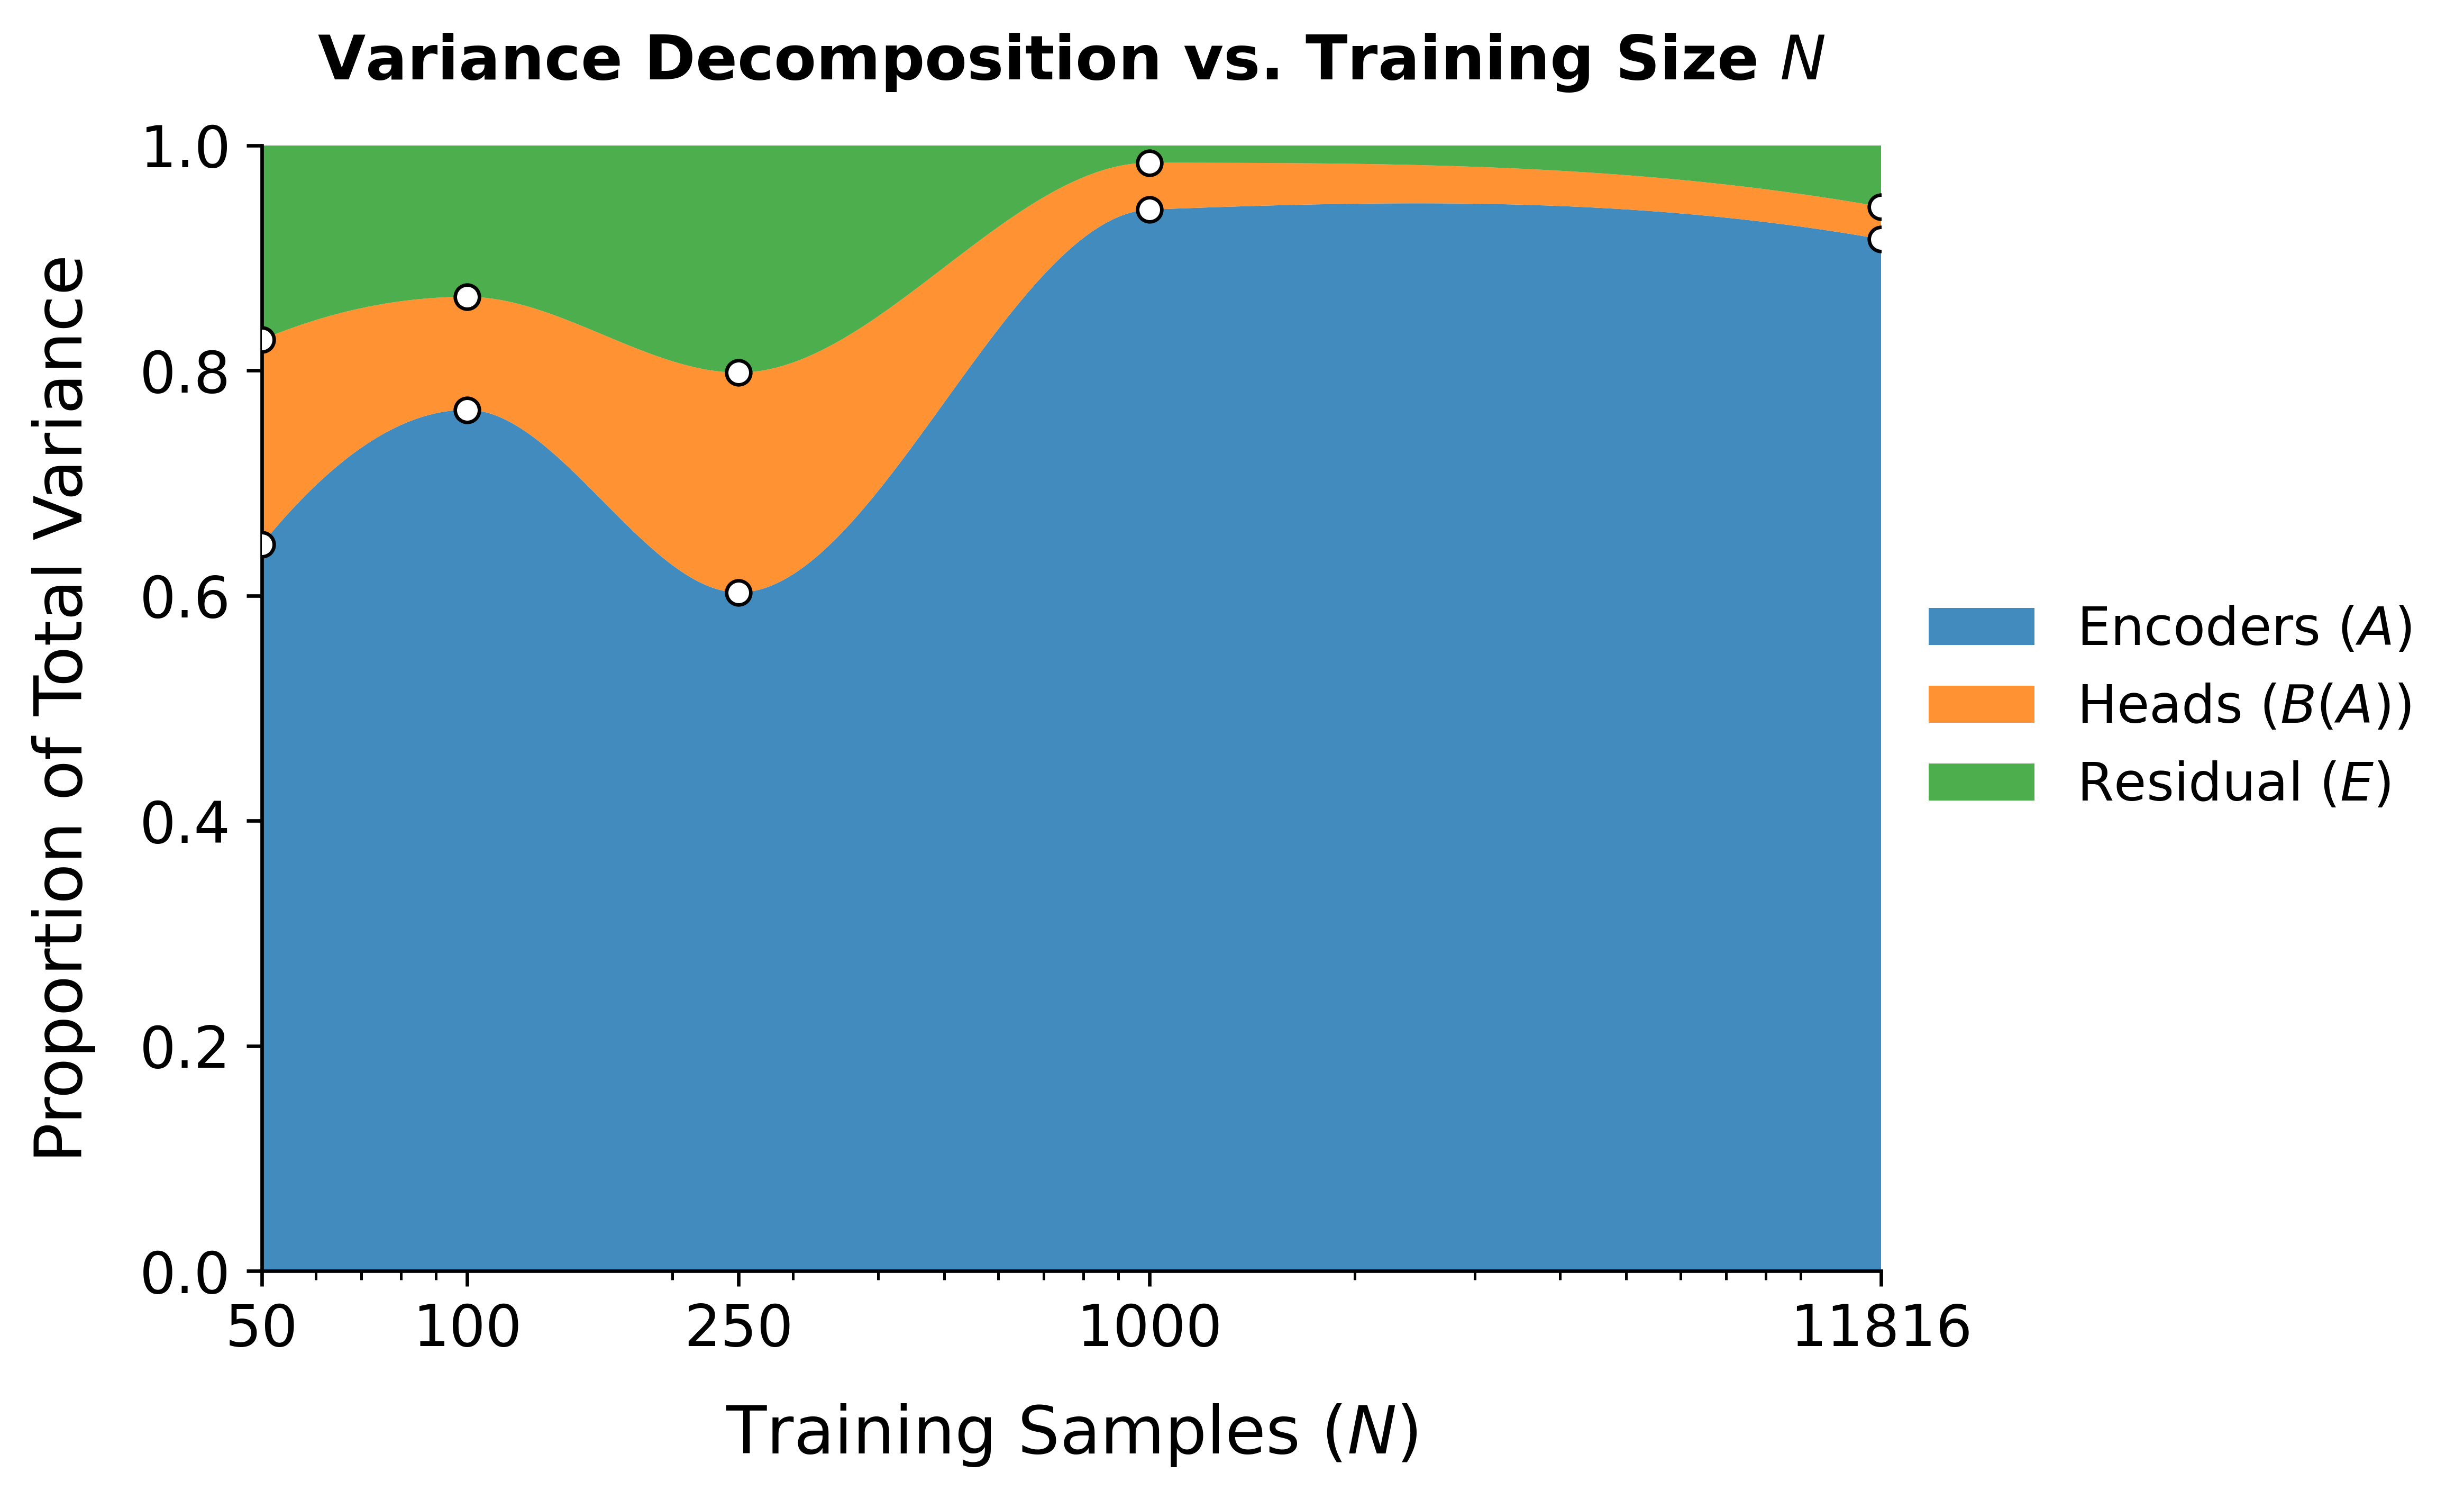
\includegraphics[width=0.9\linewidth]{figures/variance-decomp.png}
  \caption{\textbf{Proportion of total test-set RMSE variance attributable to encoder-level stochasticity, head-level variability, and residual noise.} The breakdown is shown as a function of training set size $N$ on Deep4Chem, with variance proportions estimated using a two-factor nested random-effects decomposition.}
  \label{fig:var-decomp}
\end{figure}

As $N$ increases, the contribution of the head diminishes, and predictive variability becomes dominated almost entirely by stochasticity in encoder training. This explains the convergence of hybrid and end-to-end models at scale: once the dataset is large enough to constrain the representation, the specific choice of head becomes less critical. The hybrid advantage in low-data regimes, therefore, stems from XGBoost's ability to efficiently navigate the high-variance ``head'' component of the error budget.

Uncertainty estimates for the variance components, obtained via bootstrap resampling, are reported in the Supporting Information (Table~\ref{tab:si_varcomp_bootstrap}); while confidence intervals are wide at small training set sizes, the qualitative dominance of encoder-level stochasticity is preserved across regimes.

\section{Transfer Learning and Pretraining Effects}
We next evaluate whether pretraining on the large Deep4Chem corpus can mitigate data scarcity in smaller, domain-specific tasks. We compare four strategies defined in Methods: Random Initialization, Zero-Shot Pretrained, Two-Stage Fine-Tuning, and Hybrid Transfer.

\begin{figure*}[t]
  \centering
  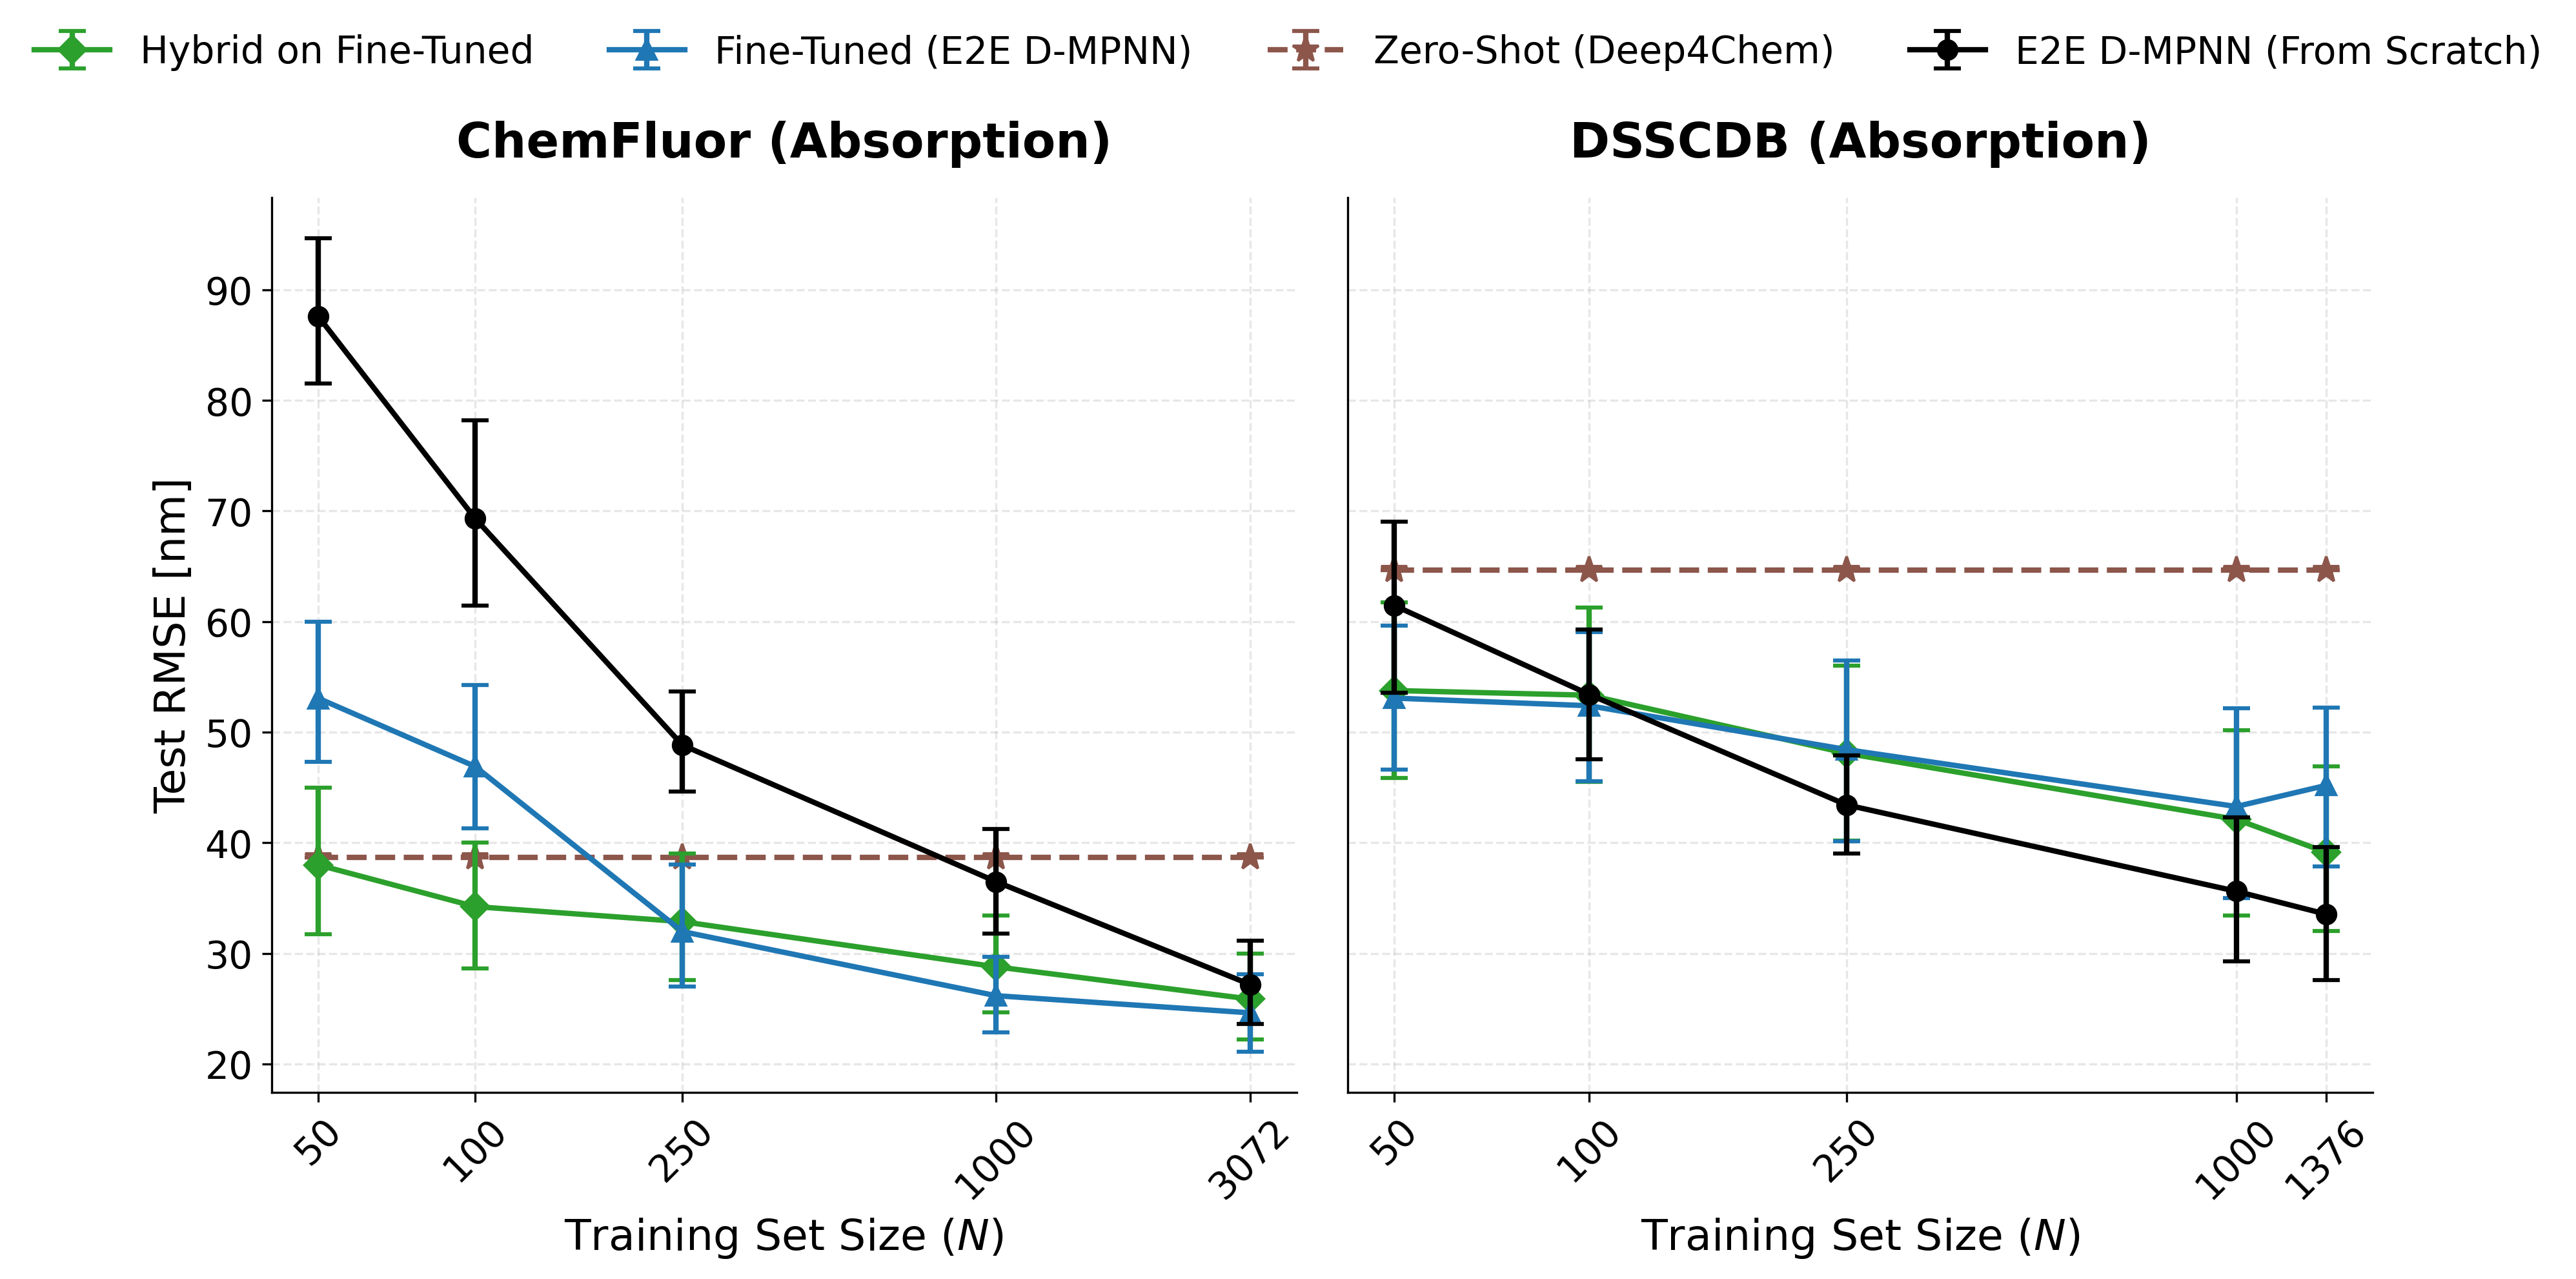
\includegraphics[width=0.9\linewidth]{figures/abs_transfer_multipanel_bootstrap.png}
  \caption{\textbf{Regime-dependent benefits of transfer learning.} 
  Test RMSE (scaffold split) versus training set size $N$ for \textbf{(A) ChemFluor} and \textbf{(B) DSSCDB}. 
  Strategies include training from scratch (black circles), two-stage fine-tuning of a Deep4Chem-pretrained encoder (blue triangles), and hybrid XGBoost head applied to fine-tuned embeddings (green diamonds). 
  The zero-shot performance of the Deep4Chem model (brown stars) is provided as a baseline. 
  Error bars indicate 95\% percentile bootstrap confidence intervals for the test RMSE, computed by resampling test molecules with replacement (2000 replicates).}
  \label{fig:transfer_multipanel}
\end{figure*}

\paragraph{Transfer to ChemFluor (High Chemical Overlap).}
Figure~\ref{fig:transfer_multipanel}A demonstrates that for ChemFluor, which shares significant structural similarity with Deep4Chem, transfer learning appears particularly effective. Fine-tuning a pretrained encoder yields substantial RMSE reductions over training from scratch in the $N \leq 1000$ regime. Notably, the Hybrid Transfer strategy on these fine-tuned embeddings provides even further improvement. This confirms that even when transfer is successful, the regularization benefits of the hybrid model persist in the ultra-low-data limit.

\paragraph{Transfer to DSSCDB (Low Chemical Overlap).}
In contrast, transfer to the DSSCDB dataset (Figure~\ref{fig:transfer_multipanel}B) illustrates the limitations of pretraining under distribution shift. DSSCDB contains distinct dye classes poorly represented in Deep4Chem. Consequently, the zero-shot baseline performs poorly, and fine-tuning offers only negligible gains at $N=50$. As data availability increases, models trained from scratch rapidly surpass the transfer-learning models. This likely reflects representational bias from pretraining.

\begin{figure}[t]
  \centering
  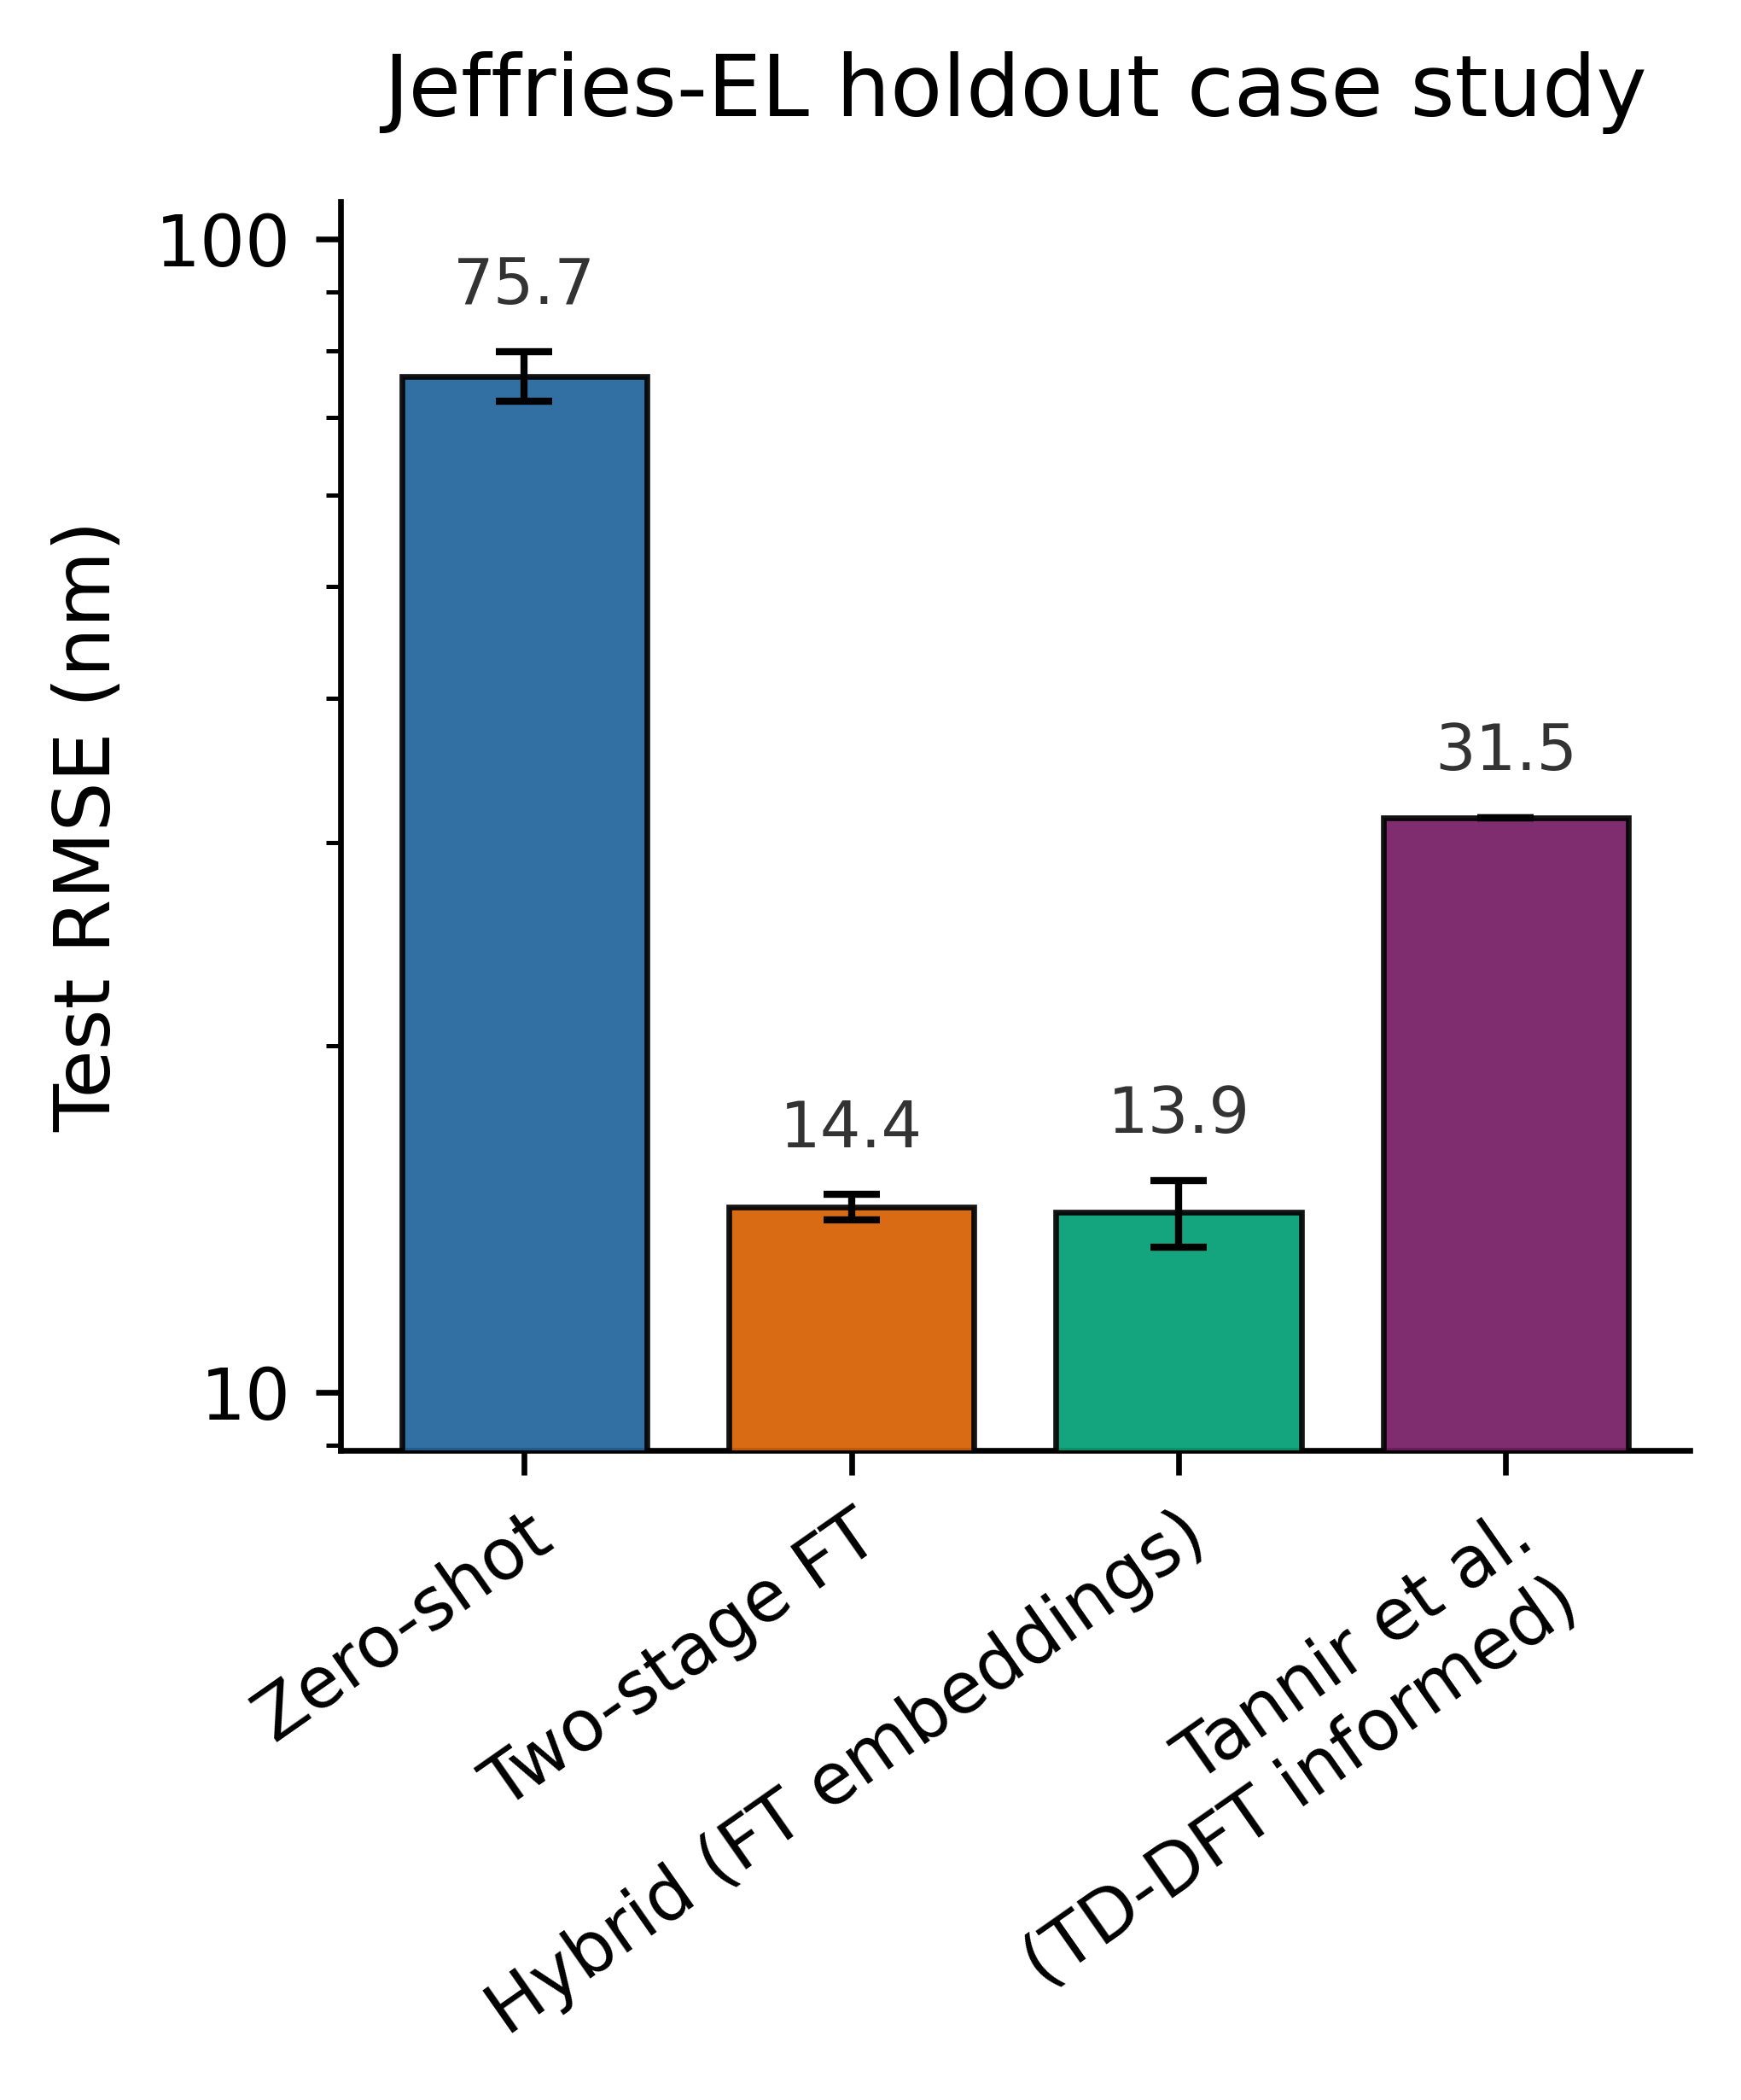
\includegraphics[width=0.5\linewidth]{figures/jeffries_case_study_bars.png}
  \caption{\textbf{Jeffries-EL Case Study ($N=43$).} Test RMSE on the holdout set. The Hybrid model trained on fine-tuned embeddings achieves the lowest error, outperforming both standard fine-tuning and domain-specific physics-informed baselines (Tannir \textit{et al.}).}
  \label{fig:jeffries_case_study}
\end{figure}

\paragraph{Case Study: Jeffries-EL (Ultra-Small $N$).}
Based on the transfer behaviours observed on ChemFluor and DSSCDB, we hypothesized that the Jeffries-EL dataset ($N=43$) would benefit significantly from pretraining due to its chemical alignment with Deep4Chem. Moreover, we anticipated that the hybrid architecture would further enhance performance by stabilizing the head in this ultra-low-data limit. The results are consistent with these expectations. Figure~\ref{fig:jeffries_case_study} shows that the hybrid transfer model achieves the lowest test RMSE, outperforming both standard fine-tuning and the domain-specific TD-DFT-informed baselines reported by Tannir \textit{et al.} on the exact same holdout set~\cite{tannir2024predicting}. This reinforces our earlier findings: when downstream chemistry aligns with the pretraining corpus, hybrid transfer learning can leverage prior knowledge to outperform even the physics-based descriptors.

\subsection{Interpretation of Learned Molecular Representations}

The D-MPNN encoder serves as a nonlinear feature extractor, mapping complex molecular graphs into high-dimensional latent representations. While such high-dimensional vectors are necessary to provide the representational capacity required for state-of-the-art accuracy, they risk becoming ``black boxes'' that obscure the underlying chemical logic \cite{yang2019analyzing, gomez2018automatic}. A critical question for any scientific ML model, particularly under data scarcity, is whether it learns physically meaningful features or merely exploits dataset statistics. To address this, we analyze the structure of the learned D-MPNN embeddings on the Deep4Chem and ChemFluor datasets using PCA and interpretable descriptors.


\paragraph{Stability of the Latent Space.}
Despite the stochasticity of training, the D-MPNN tends to converge to a stable low-dimensional manifold across encoder seeds. The PCA reveals that the resulting embedding space is relatively low-dimensional: the top 24 components capture $\sim$90\% of the variance in the 482-dimensional embedding space. By aligning the principal components across independent training seeds (using the HOMO--LUMO gap to resolve sign ambiguity), we find that the dominant axis ($PC_0$) is reproduced with high consistency across runs.

This dominant variance is closely aligned with predictive utility. Five independent auxiliary XGBoost heads trained on the seed-dependent PCA-transformed embeddings consistently identify $PC_0$ as the most influential feature, accounting for an average of $48.1\%$ of total feature importance, with remaining importance distributed across secondary axes. Complementary SHAP (Shapley Additive Explanations) analysis supports this hierarchy, indicating that the model relies primarily on the $PC_0$ axis for global spectral shifts while using higher-order components for localized adjustments (see Supporting Information Figure~\ref{fig:shap-scores}).

We observed similar semantic trends across datasets (see Supporting Information Figure~\ref{fig:chemfluor-pc-physchem-heatmap}). This replication supports the claim that the D-MPNN often learns a chemically meaningful organization aligned with known determinants, regardless of stochastic initialization or specific dataset composition.

\paragraph{Correlation with Physical and Chemical Descriptors.}
To interpret these latent directions, we examine the Spearman rank correlations between the aligned principal components and independent RDKit descriptors (Figure~\ref{fig:pc-physchem-heatmap}). These descriptors (Table~\ref{tab:chemical-descriptors}) were not provided to the model during training; the observed correlations emerge solely from the model's learned representation of the molecular graph. 

Across encoder seeds, the aligned principal components exhibit highly stable correlations with physically meaningful quantities. The dominant component ($PC_0$) is strongly correlated with both the HOMO--LUMO gap and absorption wavelength ($\rho = -0.820 \pm 0.007$ and $\rho = 0.942 \pm 0.003$, respectively). This correlation is far stronger than that of simple topological descriptors like \textit{NumConjugatedBonds} ($\rho = 0.24$). Full seed-level statistics are reported in Supporting Information Table~\ref{tab:pc0_stability_deep4chem}.


\begin{figure*}[t]
 \centering
 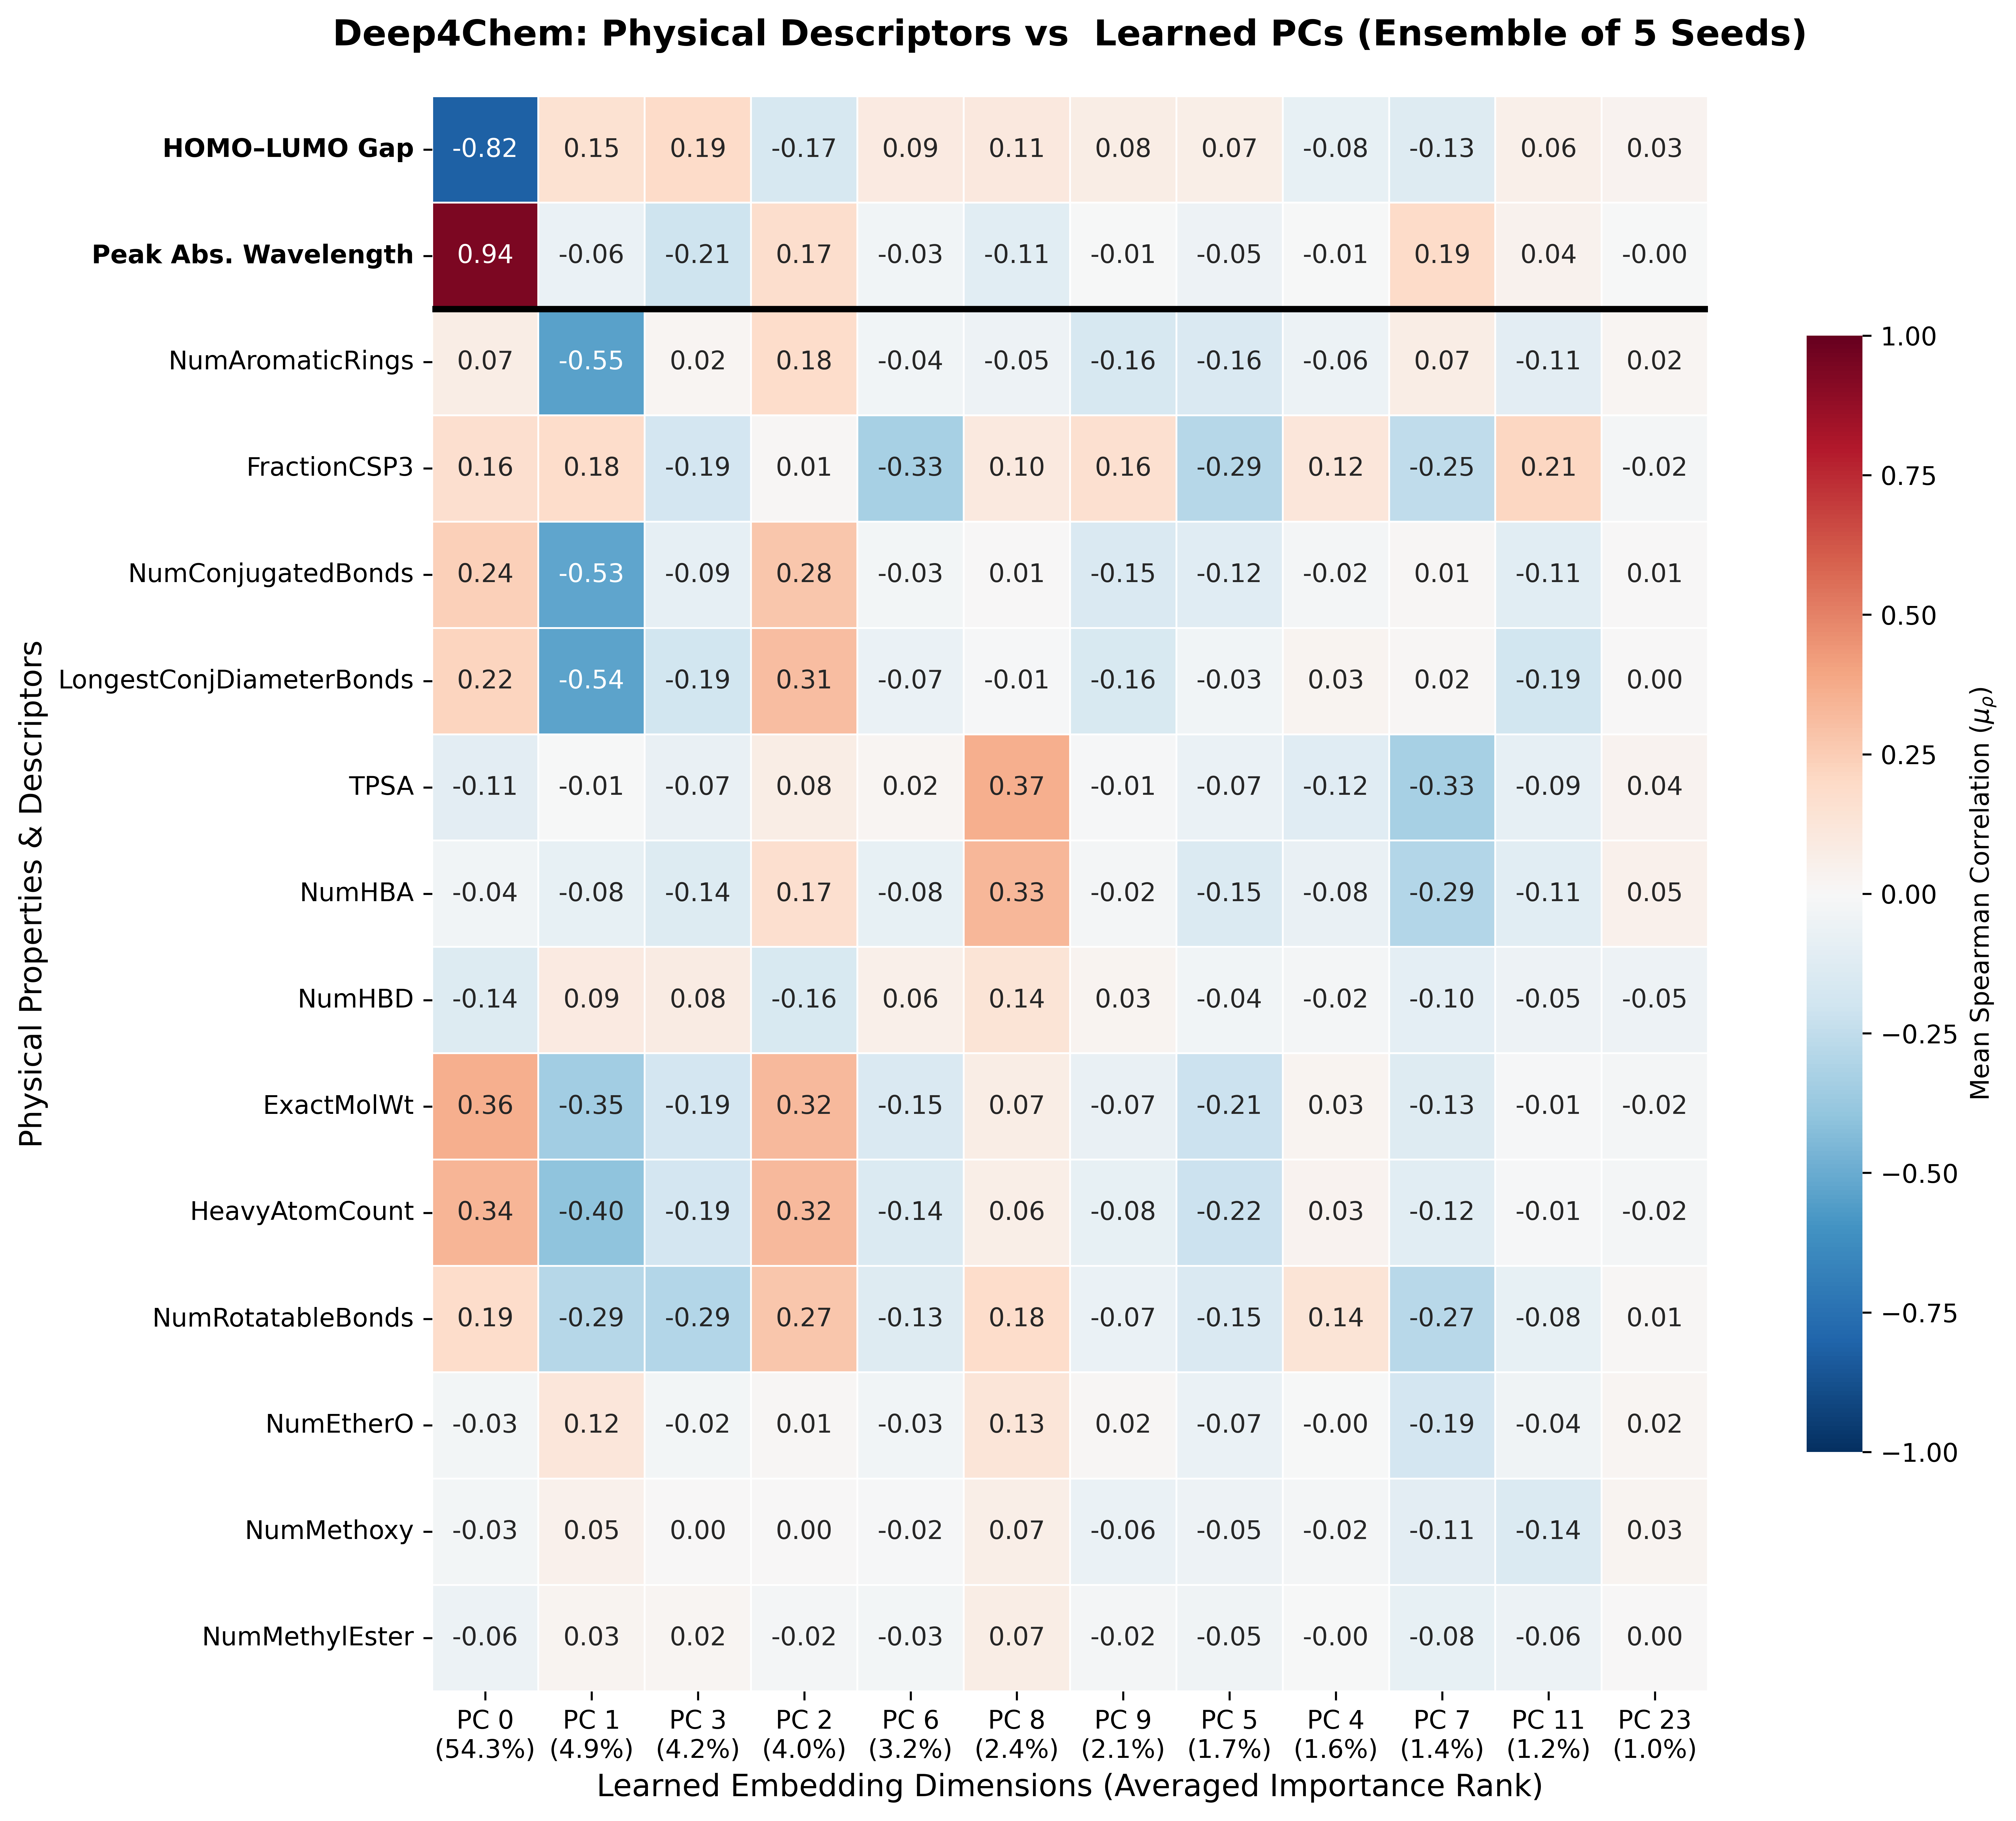
\includegraphics[width=0.8\textwidth]{figures/deep4chem-pc-physchem-heatmap.png}
\caption{\textbf{Consensus Interpretability Map: Learned PCs vs Physics.} 
Aligned Spearman rank correlations between the top 12 predictive principal components (PCs) and physicochemical descriptors across an ensemble of 5 seeds. PCs are ordered by averaged XGB feature importance. The horizontal divider separates structural descriptors from the photophysical targets, HOMO--LUMO gap and peak absorption wavelength.}
\label{fig:pc-physchem-heatmap}
\end{figure*}

\subsection{Chemical Interpretation of Principal Components}
\paragraph{$PC_0$: The Effective Conjugation Axis.}
As visualized in Figure~\ref{fig:abs-vs-pc0}, $PC_0$ can be interpreted as a learned coordinate for \textbf{``effective conjugation length''}. It separates molecules not just by the number of double bonds, but by their ability to delocalize electrons. Low $PC_0$ values correspond to torsionally twisted or interrupted $\pi$-systems, while high $PC_0$ values correspond to extended, planar architectures that promote efficient orbital overlap. The saturation of $\lambda_{\max}$ at high $PC_0$ values mirrors the physical ``saturation of redshift'' observed in long conjugated polymers~\cite{meier1997effective}, suggesting that the model has learned latent axes exhibiting behaviour consistent with known non-linear physics of delocalization without explicit supervision.

\begin{figure*}[t]
  \centering
  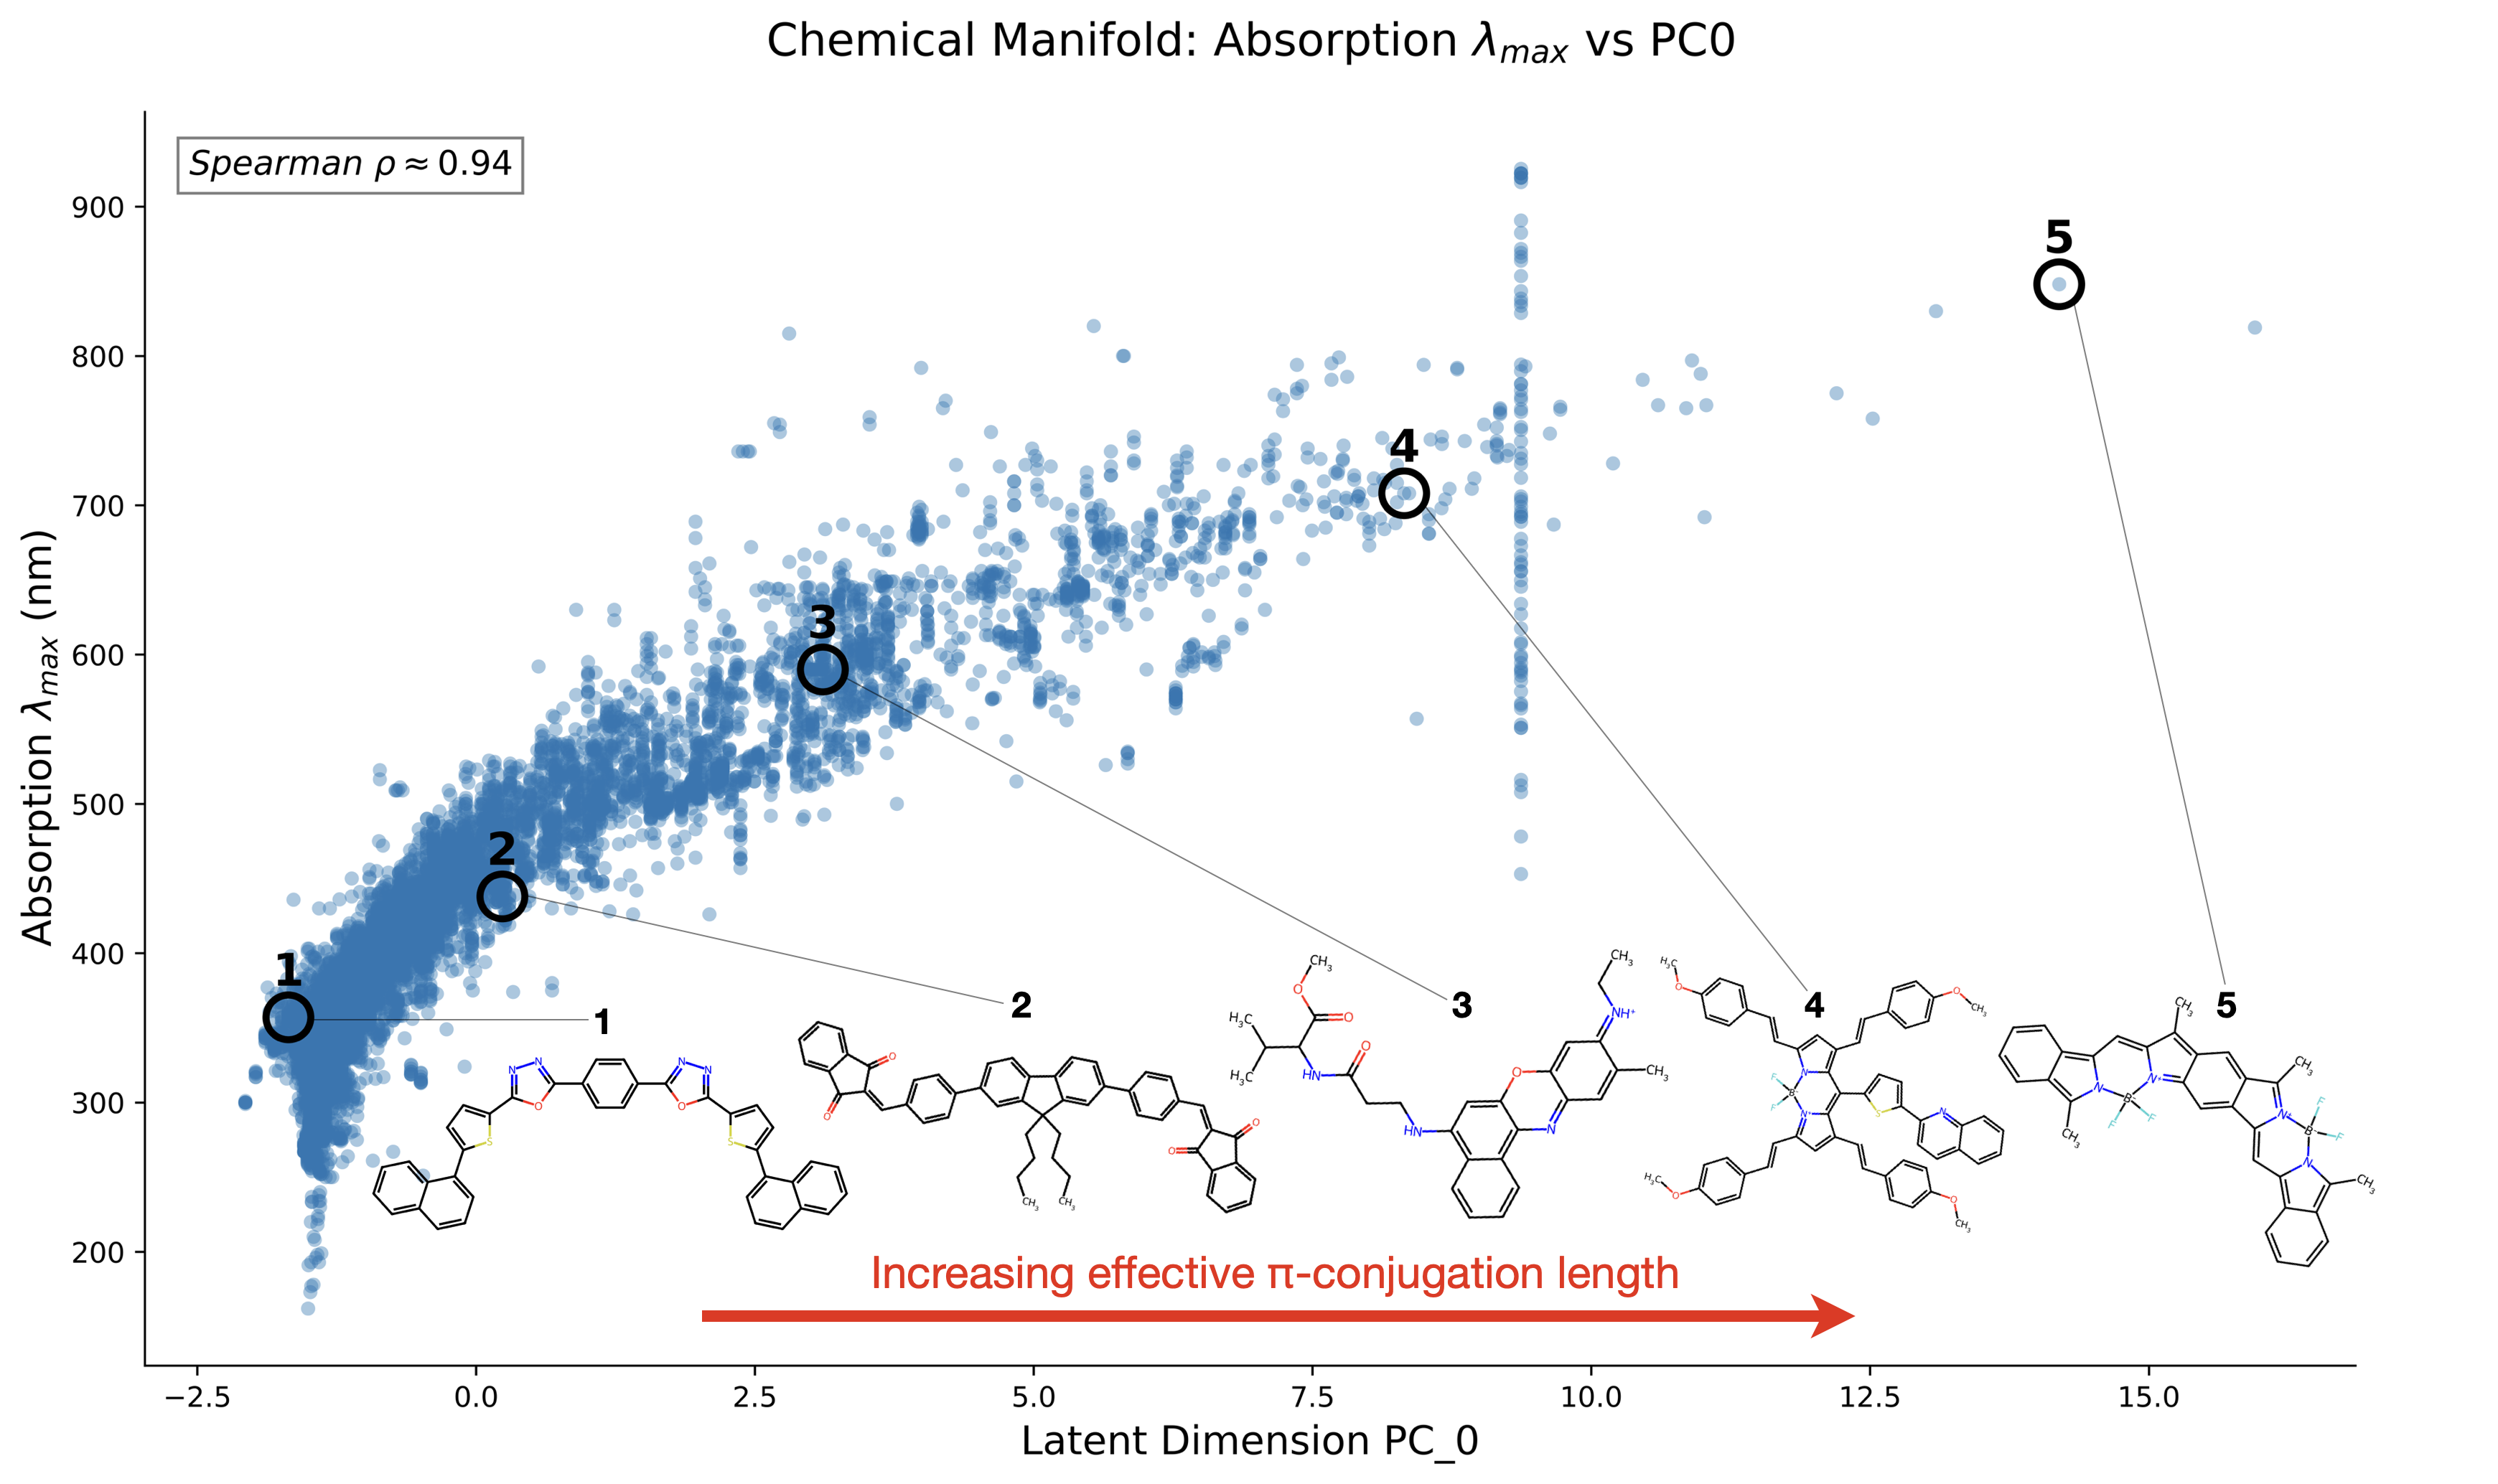
\includegraphics[width=0.9\textwidth]{figures/abs-vs-pc0.png}
  \caption{\textbf{Chemical manifold visualization showing the relationship between absorption $\lambda_{\max}$ and the dominant latent dimension $PC_0$.} The axis corresponds to ``effective conjugation length'': low values indicate interrupted or localized $\pi$-systems, while high values indicate extended, planar delocalization.}
  \label{fig:abs-vs-pc0}
\end{figure*}


\paragraph{Secondary Structural and Environmental Axes.}
Beyond the dominant electronic axis, several secondary components encode orthogonal structural and environmental factors. $PC_1$ primarily reflects aromaticity and conjugated topology, exhibiting negative correlations with \textit{NumAromaticRings} ($\rho = -0.55$) and \textit{LongestConjChain} ($\rho = -0.54$), while $PC_2$ tracks overall molecular size and flexibility, correlating with \textit{ExactMolWt} ($\rho = 0.32$), \textit{HeavyAtomCount} ($\rho = 0.32$), and \textit{NumRotatableBonds} ($\rho = 0.27$). 

Additionally, $PC_8$ appears to reflect polarity and solvation effects, correlating with topological polar surface area and hydrogen-bonding capacity. These dimensions adjust the predicted absorption wavelength around the dominant shift captured by $PC_0$, suggesting that the model distinguishes electronic delocalization from substituent-driven polarity and solvation effects (see Supporting Information, Figures~\ref{fig:si_hexbins} and~\ref{fig:pc8-vs-pc0}).

While several principal components have clear and chemically meaningful interpretations, not all latent directions exhibit strong correlations with the descriptors examined here. This is expected: PCA is a linear projection of a highly nonlinear learned representation, and individual components may encode interactions or higher-order structure not captured by standard physicochemical descriptors. The fact that multiple dominant components align so strongly with fundamental electronic and structural quantities is therefore notable. Additional analyses and tentative interpretations of lower-correlation components are provided in the Supporting Information.


\paragraph{Orthogonality of Electronic and Structural Factors.}
To examine the separation of electronic and structural effects, we perform a counterfactual analysis (Figure~\ref{fig:counterfactuals}). By projecting pairs of molecules (in a fixed solvent) that differ by single structural edits onto the aligned global $PC_0$ axis, we observe two distinct trajectories:

\begin{itemize}
    \item \textbf{Conjugation Extension and Aromatic Fusion (e.g., Bibenzyl $\to$ Stilbene; ``Broken Pentacene'' $\to$ Pentacene):} Structural edits that physically extend the conjugated network (linking double bonds or fusing aromatic rings) result in large displacements along the $PC_0$ axis, driving the expected redshift~\cite{yamaguchi2008pi, adachi1998relationship}.
    \item \textbf{Electronic Push-Pull (e.g., \textit{para}-Nitro-substitution):} Edits that induce charge transfer without extending the $\pi$-chain (e.g., donor-acceptor substitutions) produce vertical shifts in predicted $\lambda_{\max}$ (red or blue depending on the solvent), with minimal displacement along $PC_0$~\cite{yokoyama1984effects, maximo2024absorption, szatylowicz2017classical}.
\end{itemize}

These trends suggest that the latent representation separates wavelength shifts associated with the extent of $\pi$-conjugation (captured by $PC_0$) from those associated with substituent-induced charge transfer (captured by secondary dimensions), without requiring explicit physical supervision.

\begin{figure*}[t]
  \centering
  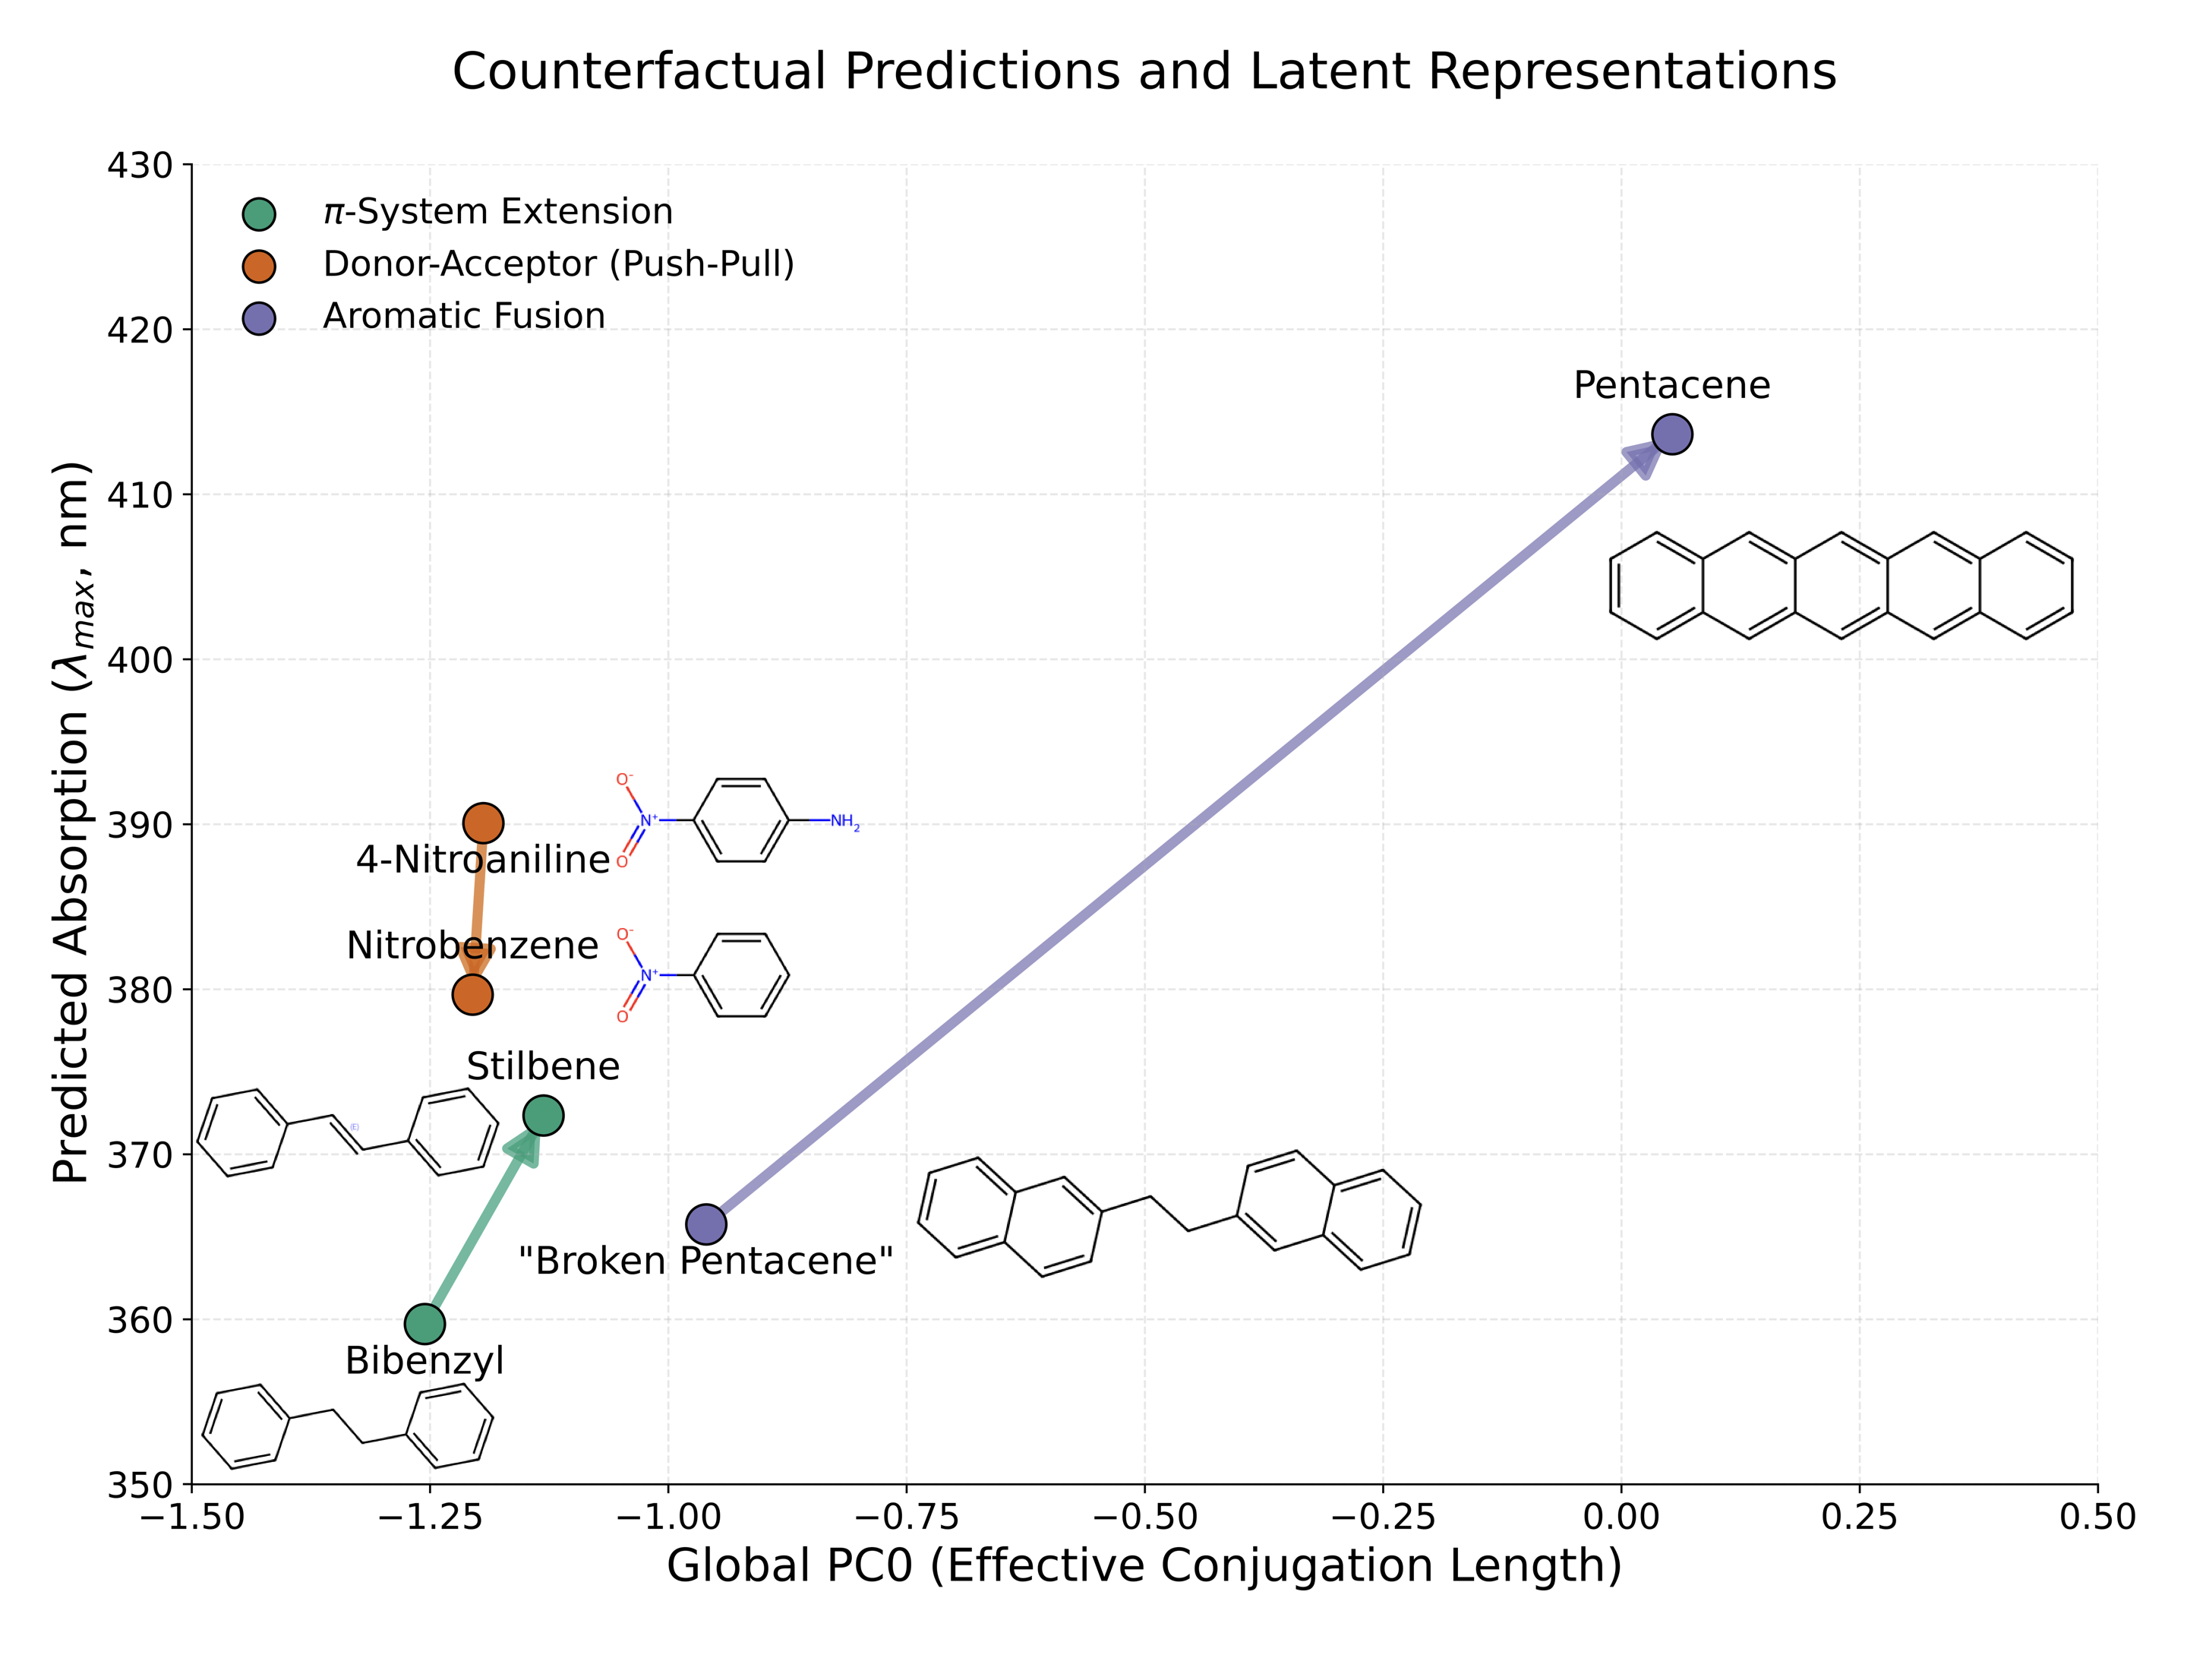
\includegraphics[width=0.9\textwidth]{figures/latent_space_interpretation_counterfactuals.png}
  \caption{\textbf{Counterfactual interpretation of the learned latent space.} 
  Latent embeddings for chemically matched pairs are projected onto the global $PC_0$ axis. Each arrow denotes a structural modification while keeping solvent constant. The horizontal axis ($PC_0$) tracks the effective conjugation length, while the vertical axis shows predicted $\lambda_{\max}$.}
  \label{fig:counterfactuals}
\end{figure*}